%--------------------------------------------------------------------------
\chapter{Tecnologias}
A escolha da maior parte das tecnologias deriva dos conhecimentos adquiridos ao longo do curso técnico de informática integrado ao ensino médio paralelamente à escolha de tecnologias proveniente de pesquisas independentes realizadas pelas integrantes da equipe. Consequentemente, tais tecnologias, quando usadas em conjunto, cumprem as necessidades e agregam positivamente no desenvolvimento do projeto. 

% DESENVOLVIMENTO -----------------------------------------------------
\section{Desenvolvimento}
As tecnologias adotadas que serão utilizadas no desenvolvimento da aplicação são:
\begin{enumerate}
\item  Para o desenvolvimento do back-end será utilizada a linguagem de programação PHP. PHP Hypertext Preprocessor, mais conhecida como PHP, é uma linguagem interpretada e open source, amplamente utilizada na criação de websites dinâmicos conjuntamente ao HTML \cite{php};
\item A IDE Visual Studio Code será utilizada como ferramenta de desenvolvimento do back-end. É um ambiente de desenvolvimento integrado da Microsoft que combina ferramentas comuns de desenvolvimento em uma única interface gráfica do usuário (GUI)\cite{ide2} para a construção e/ou manutenção de softwares, podendo-se ser utilizado em variadas plataformas (Windows, Linux e macOS)\cite{ide}; 
\item A linguagem de marcação HTML5 será utilizada para o desenvolvimento do front-end. Conforme o blog rockcontent, HTML ou Hyper Text Markup Language é a linguagem de marcação padrão da internet com textos em blocos interconectados contendo palavras, imagens, sons, tabelas e outros elementos; é utilizada em conjunto das tecnologias CSS e JavaScript para criar páginas webs \cite{html};
\item A linguagem Cascading Style Sheet (CSS) será utilizada em conjunto ao HTML para o desenvolvimento do front-end. O CSS é uma folha de estilos em cascatas utilizada para estilizar elementos escritos pela linguagem de marcação \cite{css};
\item A linguagem de programação JavaScript (JS) será utilizada paralelamente ao HTML e ao CSS para o desenvolvimento do front-end e para obter a localização atual de um usuário pelo uso do objeto \textit{geolocation}. De acordo com o site MDN Web Docs, o JS permite a implementação de itens complexos em páginas web permitindo a criação de conteúdos que atualizam-se dinamicamente e controlar multimídias, mapas interativos, gráficos 2D/3D animados, etc \cite{js};
\item O framework Bootstrap 4 será utilizado em conjunto do HTML, CSS e JavaScript para o desenvolvimento do front-end. É um framework que de código-aberto que possui integração com qualquer linguagem de programação tornando possível uma otimização do desenvolvimento da plataforma através da adoção de uma estrutura única, reduzindo inconsistências entre as diversas formas de se codificar, que variam de profissional para profissional \cite{bootstrap};
\item A ferramenta PostgreSQL será utilizada para as configurações do banco de dados. Segundo o blog rockcontent, é um sistema de gerenciamento de banco de dados relacionados que tem por objetivo permitir a implementação da linguagem SQL em estruturas, garantindo um trabalho com os padrões desse tipo de ordenação dos dados \cite{postgre}.
\end{enumerate}
%--------------------------------------------------------------------------

% HOSPEDAGEM CLOUD -----------------------------------------------------
\section{Hospedagem Cloud}
Inicialmente, para a hospedagem em nuvem da aplicação, a equipe optou pelo uso do 000Webhost, um serviço de hospedagem gratuito controlado pela empresa Hostinger por ser um serviço que disponha de mais informações disponíveis.  \cite{hospedagem1, hospedagem2}. 

A segunda opção testada da equipe foi o Heroku, uma dica dos professores Ivan Martinez e Leonardo Motta, sendo é uma plataforma em nuvem gratuita que oferece uma gama de serviços que permitem aos desenvolvedores a implementação, escalonamento e gerenciamento de aplicações. Entretanto, o Heroku estava gerando certificado SSL (Secure Sockets Layer) nota B. \cite{heroku}. 

Para atender, assim, o requisito dos professores da disciplina técnica Prática de Desenvolvimento de Sistemas (PDS) em relação ao certificado SSL com nota A, a equipe passou a utilizar o Azure – a plataforma em nuvem da empresa Microsoft. Este fornece um plano gratuito pela parceiria do Instituto Federal de São Paulo (IFSP) com a Microsoft. 

%--------------------------------------------------------------------------

% ORGANIZACAO E GERENCIAMENTO -----------------------------------------------------
\section{Organização e Gerenciamento}
Os professores da disciplina técnica PDS definiram, como repositório oficial, o sistema de controle de versão Subversion (SVN) – cuja funcionalidade é gerenciar diferentes versões no desenvolvimento de um documento. A ferramenta open-source Gource será utilizada para a visualização do desenvolvimento do projeto, a qual tem base no SVN.

A equipe fará uso do LaTeX – um programa de marcação para a edição de documentos de alta qualidade tipográfica – para que o corpo do documento mantenha-se padronizado. Este programa também foi predefinido pelos professores da disciplina técnica PDS. 
%--------------------------------------------------------------------------
%----------------------------------------------------------------------
\chapter{Diagrama de arquitetura}
De acordo com Ionut Balosin em seu artigo \textit{Por que precisamos de diagramas de arquitetura?} – traduzido por Marcelo Costa, o principal objetivo dos diagramas arquiteturais é facilitar a colaboração, comunicação, visão e orientação dentro da equipe, ou seja, os diagramas de arquitetura devem ajudar a todos a ver o panorama e entender o ambiente \cite{diagrama}. Na \autoref{fig_diagrama} é possível observar o diagrama de arquitetura da aplicação web PETINDER.
%--------------------------------------------------------------------------
\begin{figure}[htb]
    \centering
	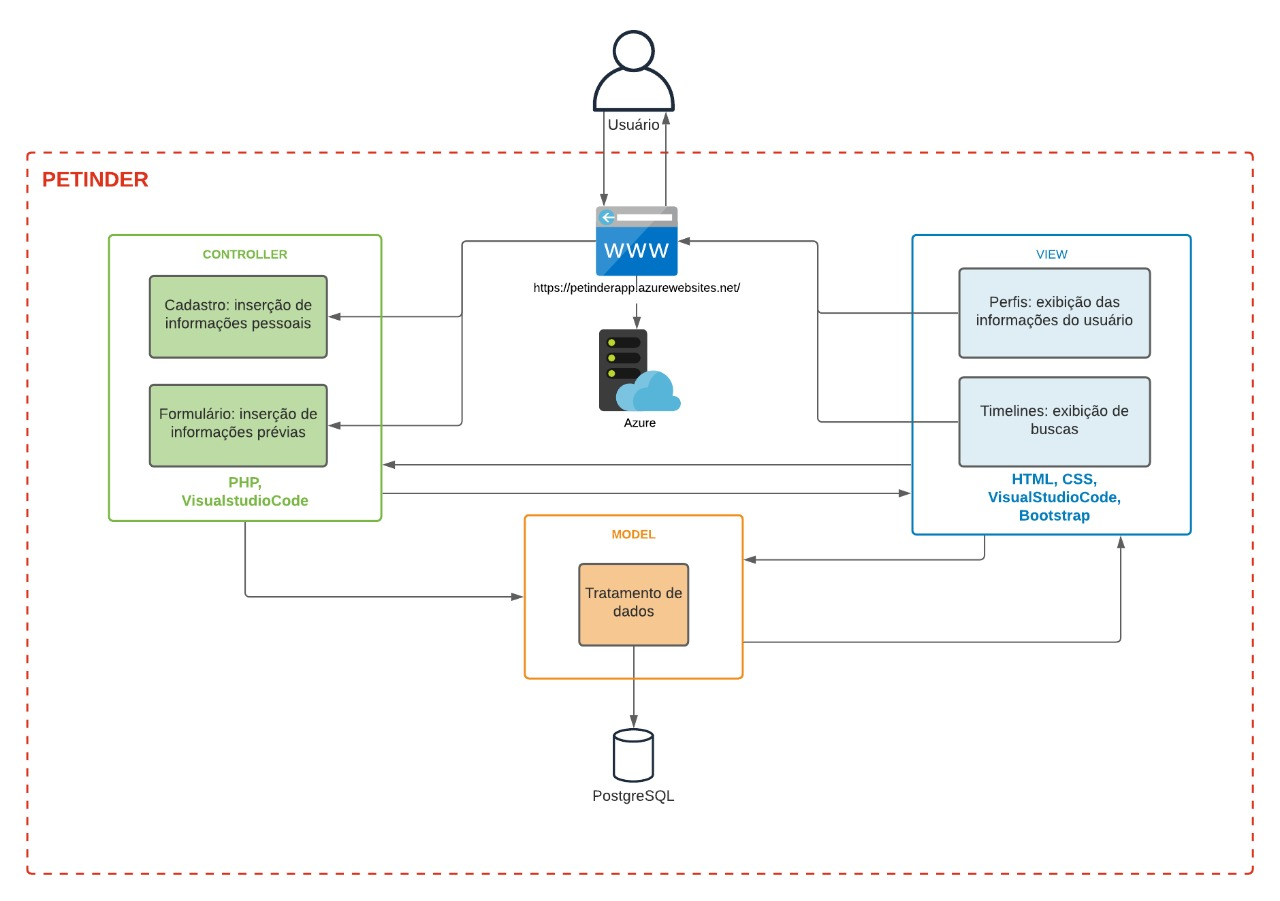
\includegraphics[width=1\textwidth]{imagens/diagrama_de_arquitetura.jpg}
	\caption{\label{fig_diagrama}Diagrama de arquitetura do sistema}
	\fonte{Elaborada pelos autores}
\end{figure}

% ---
% Conclusão (outro exemplo de capítulo sem numeração e presente no sumário)
% Dependendo do trabalho desenvolvido ele pode ter uma Conclusão ou Considerações finais
% Para trabalhos de disciplina utilizar Considerações Finais
% ---
\chapter*{Considerações Finais}

%--------------------------------------------------------------------------
%--------------------------------------------------------------------------